%
% introduction.tex
%
% Copyright (C) 2020 by SpaceLab.
%
% PC-104 Adapter Documentation
%
% This work is licensed under the Creative Commons Attribution-ShareAlike 4.0
% International License. To view a copy of this license,
% visit http://creativecommons.org/licenses/by-sa/4.0/.
%

%
% \brief Introduction chapter.
%
% \author Gabriel Mariano Marcelino <gabriel.mm8@gmail.com>
%
% \institution Universidade Federal de Santa Catarina (UFSC)
%
% \version 2.0.0
%
% \date 2020/06/21
%

\chapter{Introduction} \label{ch:introduction}

The PC-104 Adapter boards are intended to be used in 2 or 3U CubeSat structures as an interconnection of two PC-104 bus segments. This interconnection is made with a set of PicoBlade \cite{picoblade} cables between the top and bottom boards. The set of two boards (top and bottom) of the adapter can be seen in \autoref{fig:pc104-adapter}.

\begin{figure}[!htb]
    \begin{center}
        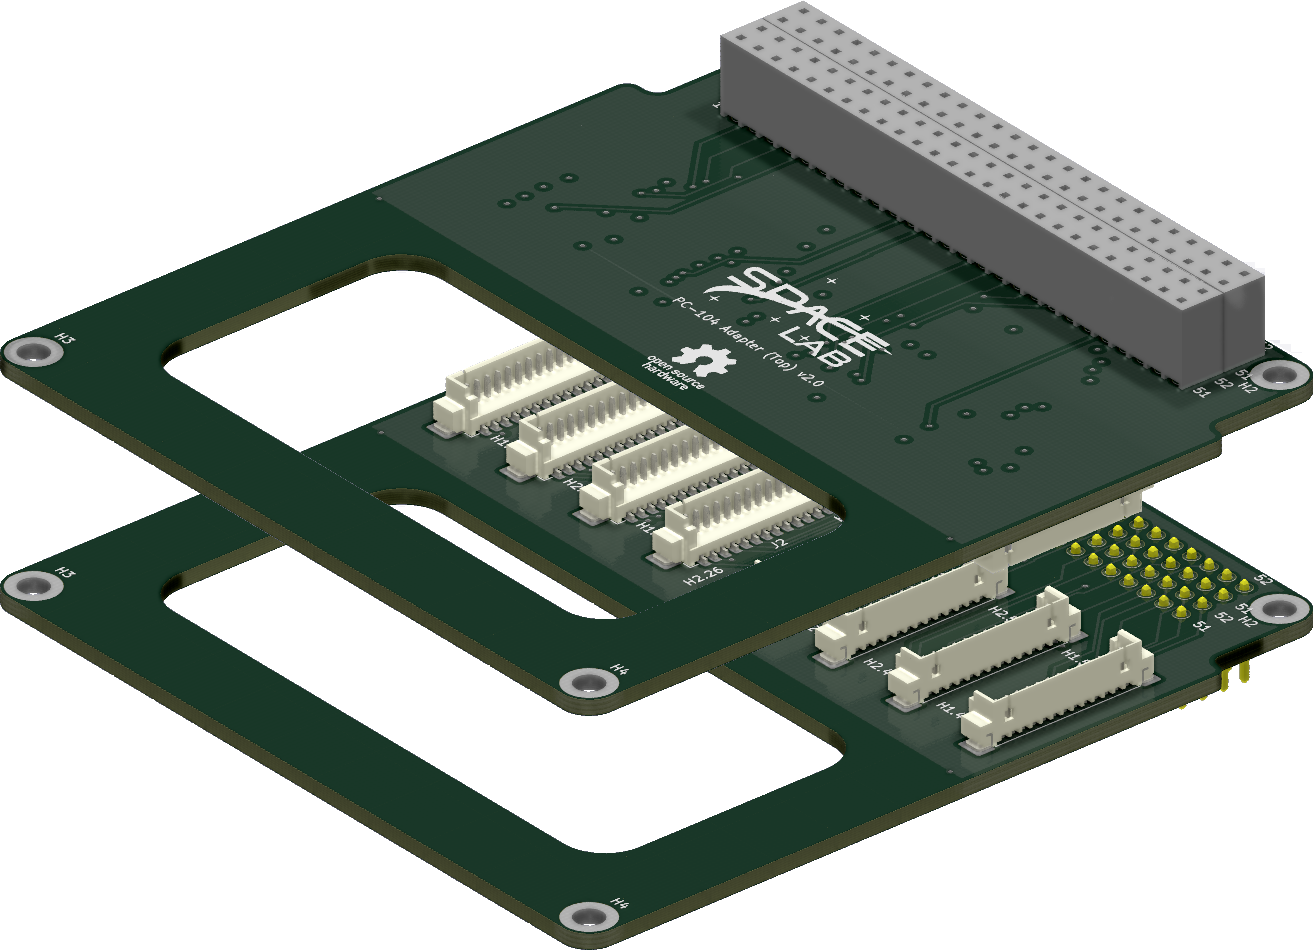
\includegraphics[width=0.7\textwidth]{figures/pc104-adapter}
        \caption{PC-104 adapter boards.}
        \label{fig:pc104-adapter}
    \end{center}
\end{figure}

This adapter was designed with the objective of be used in the GOLDS-UFSC mission \cite{golds-ufsc}, but it is possible to reuse it others mission with similar characteristics (2 or 3U structures divided in segments).

The project is open and licensed under the CERN Open Hardware License, version 2 (CERN OHL-S 2). The source files and this document are available in \cite{pc104-adapter}.
